\documentclass[a4paper,12pt,french]{article}

\usepackage[utf8]{inputenc}
\usepackage[T1]{fontenc}
\usepackage[upright]{kpfonts}

\usepackage{amsmath,amsfonts,amssymb}
\usepackage[margin=1.4cm]{geometry}
\usepackage{hyperref}
\usepackage{enumitem}
\usepackage{multicol}
\usepackage{esvect}
\usepackage{array}
\usepackage{tikz}
\usetikzlibrary{babel}
\usepackage{babel}

\setlength{\columnseprule}{0pt}
%\setlength{\parindent}{0pt}
\setlist{noitemsep}
%\setlist[1]{\labelindent=\parindent} % < Usually a good idea
\setlist[itemize]{leftmargin=*}
\setlist[itemize,1]{label=$\blacktriangleright$}
\setlist[enumerate]{labelsep=*, leftmargin=1.5pc}
\setlist[enumerate,1]{label=\arabic*., ref=\arabic*}
\setlist[enumerate,2]{label=\emph{\arabic*}),
ref=\theenumi.\emph{\arabic*}}
\setlist[enumerate,3]{label=\roman*), ref=\theenumii.\roman*}
\setlist[description]{font=\sffamily\bfseries}

\newcommand{\N}{\mathbf{N}}
\newcommand{\R}{\mathbf{R}}
\newcommand{\abs}[1]{\left\lvert #1\right\rvert}
\newcommand{\norme}[1]{\left\lVert #1\right\rVert}
\newcommand{\Vect}[2]{\left(\begin{array}{c}#1\\#2\end{array}\right)}

\title{Conseils et compétences à avoir pour aborder la terminale}
\author{\textsc{Jumel}}
\date{août 2017}

\begin{document}

\maketitle

\begin{abstract}
  Ce document est un résumé du programme, bâti et ordonné à partir de
  celui-ci, à l'exception des points sur l'algorithmique et sur la
  logique et l'écriture mathématique qui ont été replacé au début.

  Ce document ne doit pas se lire comme un article de journal, mais
  crayon et brouillon à proximité. En effet, des exercices l'émaille et
  leur résolution est vivement recommandée. Certains sont de simples
  exercices (\emph{savoir faire}) d'autres sont des démonstrations
  (\emph{savoirs}) qui peuvent être réutilisées dans d'autres contextes.
\end{abstract}

\tableofcontents

\pagebreak

\section{Langage, logique et expression}

\subsection{Langage mathématique}

Traduire à l'aide d'une phrase en français les expressions suivantes
écrite dans le langage mathématiques :
\begin{itemize}
  \item $x$ est un nombre entier supérieur ou égal à 2 ;
  \item il existe une fraction égale à $\sqrt{2}$ ;
  \item l'ensemble des nombres entiers inférieurs à $A$ ;
  \item $x$ appartient à l'ensemble des nombres réels compris entre 1 et
    $\pi$ ;
\end{itemize}

\subsection{Logique}

Parmi les affirmations suivantes, indiquez les quelles sont justes, et
sinon, proposer une correction.
\begin{itemize}
  \item $a<b \iff a^2 < b^2$
  \item $k < n \iff k - 1 \leqslant n$
  \item $k < n \iff k \leqslant n - 1$
  \item $A$ et $B$ sont deux parties de $E$ un ensemble, si $x \not\in
    A$ alors $x\in B$.
\end{itemize}

\subsection{S'exprimer pour convaincre (et non persuader)}

Un des buts finaux de l'enseignement des mathématiques au lycée est
l'acquisition par tous des éléments qui permettront un choix éclairé et
permettront une communication scientifique des résultats. Il est
important de noter que cette capacité à enchaîner logiquement des
propositions, afin de convaincre le lecteur du bien fondé de son
affirmation finale.

Celle-ci ne prendra toute sa puissance qu'à l'aide de définition
rigoureuse des «objets» considérés par notre étude. Cette rigueur est ce
qui doit animer en tout point l'écriture des mathématiques.

Cette écriture est souvent facilité et réduite (dans le but de lever des
ambiguïtés) en utilisant un formalisme particulier.

\section{Algorithmique}

En ce qui concerne les algorithmes, il faut être capable :
\begin{itemize}
  \item écrire un algorithme issu d'un calcul ;
  \item écrire un programme, dans le langage de votre choix, permettant
    le calcul de la valeur d'une fonction ;
  \item programmer un calcul itératif, le nombre d'itérations étant
    connu à l'avance.
  \item programme une instruction conditionnelle, éventuellement dans
    une boucle.
\end{itemize}

\section{Analyse}

\subsection{Second degré}

Pour les équations suivantes, indiquer la méthode la plus adaptée à la
résolution, puis résoudre :
\begin{multicols}{4}
  \begin{enumerate}
    \item $x^2 + 2x + 1 = 0$
    \item $3x^2 + 4x + 1 = 0$
    \item $4x^2 - 4x + 1 = 0$
    \item $x^2 + 2x -1 =0$
    \item $7x^2 -3x -4 =0$
    \item $7x^2 -3x +4 =0$
    \item $x^2 - 3x -2 =0$
    \item $x^2 - 5x + 6 =0$
  \end{enumerate}
\end{multicols}
Les questions précédentes n'ont pas du prendre plus de deux minutes.

On se donne désormais un polynôme sous la forme $ax^2 + bx +c =0$,
retrouver la démonstration permettant d'obtenir la forme canonique de ce
polynôme. Expliciter pourquoi on appelle cette forme «canonique» et
comment on dégage le discriminant.

\emph{Pour les 8 polynômes précédents, donner leur signe et leurs
variations (aucune justification n'est attendue.)}

\subsection{Étude de fonctions}

Il ne faut pas perdre de vue le caractère essentiel d'une fonction qui
est une correspondance entre deux ensembles, et qui a un élément du
premier, mettons $E$, fait correspondre un unique élément de $F$. On
peut ainsi définir des fonctions qui associent à des lettres des
numéros, où qui associent à des lettres d'autres lettres ou des dessins,
ou encore autre chose.

Parmi les fonctions, on distingue les fonctions numériques, qui peuvent,
partiellement au moins, se représenter à l'aide d'une courbe, dite
courbe représentative de la fonction. Cette courbe peut présenter des
discontinuités, ou des points particuliers correspondant à un
changement de direction brusque.

\emph{Dessiner une représentation graphique pour la fonction $f$,
  croissante sur l'intervalle $[0;1[$, décroissante sur $[1,2[$,
croissante sur $[2;3[$, décroissante sur $[3;4]$.}

    \emph{Expliciter la courbe représentative de la fonction $x\mapsto
    \abs{x}$}

Soient $x$ et $y$ deux nombres réels, une seule de ces trois
propositions est vraie :
\begin{multicols}{3}
  \begin{enumerate}
    \item $\abs{x} + \abs{y} = \abs{x+y}$
    \item $\abs{x} + \abs{y} \geqslant \abs{x+y}$
    \item $\abs{x} + \abs{y} \leqslant \abs{x+y}$
  \end{enumerate}
\end{multicols}

\emph{Préciser les comparaisons possible entre $x$, $x^2$ et $\sqrt{x}$
en indiquant clairement les intervalle sur lesquels elles sont
valables.}

Soit $u$ une fonction dont on connaît les variations, préciser les
variations de $u + k$, $\lambda u$, $\sqrt{u}$ et $\frac1u$.

La démonstration de la croissance de l'application $\sqrt{\cdot}$ est un
attendu du programme.

On peut aussi démontrer que pour $0\leqslant x \leqslant 1$, $x^2
\leqslant x \leqslant \sqrt{x}$, l'inégalité étant lue «dans l'autre
sens» si $x \geqslant 1$.

\emph{Si de plus, $v$ est une autre fonction dont on connait les variations,
peut on obtenir les variations de $uv$ ? de $u+v$ ?}

\subsection{Dérivation}

La dérivée est présentée comme une limite sur un taux d'accroissement,
on doit cependant être capable de retrouver certains résultats du cours.

Bien qu'elles ne figurent pas explicitement au programme de Première,
ces démonstrations constituent un bon entraînement aux manipulations
algébriques ; démontrer que la dérivée de $x\mapsto x^n$ est la
fonction $x\mapsto nx^{n-1}$ pour tout entier naturel $n$, de même avec
les autres fonctions usuelles ($x\mapsto x,\ x\mapsto \dfrac1x,\ x\mapsto
\sqrt{x}$.)

Il est nécessaire de ne pas oublier l'interprétation graphique du taux
d'accroissement :
\begin{center}
  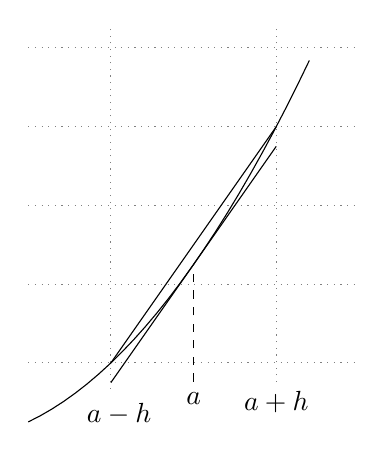
\begin{tikzpicture}[xscale=2.1,yscale=1]
    \draw [gray,dotted] (0.5,0.25) grid (2.5,5.25) ;
    \draw plot[domain=0.5:2.2] (\x,\x*\x) ;

    \draw (1,1) -- (2,4) ;
    \draw[dashed] (1.5,0.55) node[fill=white] {$a$} -- (1.5,2.25) ;
    \draw (1.5,2.25) -- +(0.5,1.5) ;
    \draw (1.05,.35) node[fill=white] {$a - h$} ;
    \draw (1.5,2.25) -- +(-1/2,-3/2) ;
    \draw (2,.5) node[fill=white] {$a + h$} ;
  \end{tikzpicture}
\end{center}

\emph{Démontrer que dans la figure ci-dessus, la «corde symétrique» par
rapport à $a$, arbitrairement choisi permet bien d'exprimer le nombre
dérivé (comparer $\dfrac{f(a+h) - f(a-h)}{2h}$ et $\dfrac{f(a+h') -
f(a)}{h'}$ et conclure.)}

\emph{Démontrer (facile) que la dérivée de la somme est la somme des dérivées
et (plus dur) que la dérivée d'un produit de deux fonctions dérivables
$u$ et $v$ est $(uv)' = u'v + uv'$.}

Utiliser ce résultat précédent pour démontrer que :
\begin{itemize}
  \item $\left(\dfrac1u\right)' = - \dfrac{u'}{u^2}$
  \item $\left(x\mapsto\dfrac1x\right)' = -\dfrac1{x^2}$
  \item $\left(x\mapsto\sqrt{x}\right)' = \dfrac1{2\sqrt{x}}$
  \item $\left(\dfrac{u}{v}\right)' = -\dfrac{u'v - v'u}{u^2}$
\end{itemize}
où $u$ et $v$ sont des fonctions dérivables et $u$ et $v$ ne sont pas
identiquement nulles, c'est à dire qu'il existe $a<b$ tels que $\forall
x\in[a;b],\ u(x) \neq 0\ \text{et}\ v(x)\neq0$.

Ces démonstrations seront revues au cours de l'année, pas de panique si
vous n'arrivez pas à les faire.

Enfin, il est utile de savoir démontrer (ici justifier à vrai dire)
pourquoi si $f$ est croissante sur un intervalle $[a;b],\ a<b$, alors
$f'x)\geqslant 0$ sur $]a;b[$. On admet la réciproque.

\subsection{Suites}

Attention aux notations ici ! On retrouve une analogie avec les
notations sur les fonctions : $f$ désigne la fonction (dans sa
globalité) et $f(x)$ est la valeur de la fonction en $x$. Ce dernier
«objet» est un nombre. Il en va de même pour les suites ; celles-ci se
notent $u$ ou $(u_n)_{n\in\N}$ dans leur globalité de suite et $u_n$
est un élément de la suite (c'est un nombre si la suite est numérique).

Donner la démonstration de la somme des $n$ premiers termes d'une suite
arithmétique de raison 1 ; de la somme des $n+1$ premiers termes d'une
suite géométrique de raison $q$.

\section{Géométrie}

\subsection{Géométrie plane}

Il est impératif de connaître ici les théorèmes de géométrie du collège,
leurs versions traditionnelles, ainsi que leur version «vectorielle».

\emph{Énoncer les théorèmes de Pythagore et de Thalès en version
«vectorielle».}

Les transformations géométriques du plan, à l'exclusion de l'homothétie,
sont des isométries. Cependant, il est utile pour ces transformations de
savoir les caractériser, aussi bien dans le langage «naturel» que dans
le formalisme vectoriel.

Au niveau du formalisme, il faut être capable de passer de l'expression
$\exists k\in\R^*,\ \vv{u} = k\vv{v}$, expression «vectorielle» de la
colinéarité à son expression analytique : $xy' - x'y = 0$ où $\vv{u} :
\Vect{x}{y}$ et $\vv{v}: \Vect{x'}{y'}$.

Cette condition et la démonstration associée permettent de déterminer :
\begin{itemize}
  \item une équation cartésienne de droite connaissant un vecteur
    directeur et un point ;
  \item un vecteur directeur d'une droite définie par une équation
    cartésienne.
\end{itemize}

\subsection{Trigonométrie}

La connaissance de la figure suivante et du tableau des valeurs
remarquables est une nécessité !

\begin{center}
  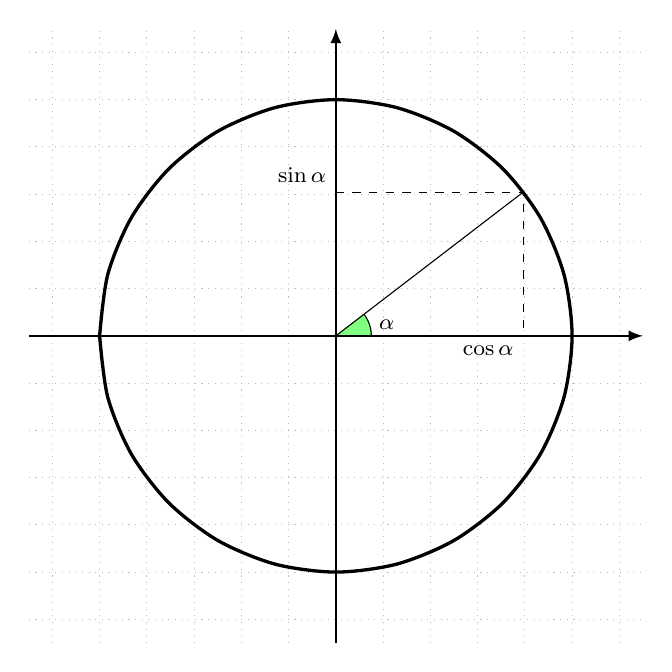
\begin{tikzpicture}[scale=3,>=latex]
    \draw [lightgray,dotted] (-1.3,-1.3) grid [step=0.2] (1.3,1.3) ;

    \def\a{37.5} \def\ca{{cos(\a)}} \def\sa{{sin(\a)}}
    \def\s{0.15}
    \draw[fill,green!50!white] (0,0) -- (\s,0) --
    plot[smooth,domain=0:\a] ({\s*cos(\x)}, {\s*sin(\x)}) -- (0,0) ;
    \draw plot[smooth,domain=0:\a] ({\s*cos(\x)}, {\s*sin(\x)}) ;
    \draw (0,0) -- ({cos(\a)},{sin(\a)}) ;
    \draw (\a/2:\s) node [right] { \footnotesize $\alpha$ };

    \draw [dashed] (0,\sa) node[above left] { \footnotesize $\sin\alpha$
    } -- (\ca,\sa) -- (\ca,0) node [below left] { \footnotesize
    $\cos\alpha$ } ;

    \draw [thick,->] (-1.3,0) -- (1.3,0) ;
    \draw [thick,->] (0,-1.3) -- (0,1.3) ;
    \draw [very thick] plot [smooth,domain=-3.14:3.14] ({cos(\x
    r)},{sin(\x r)}) ;
 \end{tikzpicture}
\end{center}

Cette figure est essentielle ; on en déduit les égalités suivantes, à
compléter pour tout angle $\alpha$ :
\begin{multicols}{4}
  \begin{itemize}
    \item $\cos\left( - \alpha\right) = \dots $
    \item $\cos\left(\alpha+\frac{\pi}2\right) = \dots $
    \item $\cos\left(\alpha-\frac{\pi}2\right) = \dots $
    \item $\cos\left(\alpha\pm\pi\right) = \dots $
    \item $\sin\left( - \alpha\right) = \dots $
    \item $\sin\left(\alpha+\frac{\pi}2\right) = \dots $
    \item $\sin\left(\alpha-\frac{\pi}2\right) = \dots $
    \item $\sin\left(\alpha\pm\pi\right) = \dots $
  \end{itemize}
\end{multicols}

On peut aussi compléter le tableau suivant des valeurs remarquables :
\begin{center}
  \renewcommand{\arraystretch}{1.2}
  \begin{tabular}{|l|*{5}{>{\hfill}p{1cm}<{\hfill~}|}}\hline
    $\alpha$     & 0 & $\frac\pi6$ & $\frac\pi4$ & $\frac\pi3$ & $\frac\pi2$ \\ \hline
    $\sin\alpha$ &   &             &             & & \\ \hline
    $\cos\alpha$ &   &             &             & & \\ \hline
  \end{tabular}
\end{center}

Ce tableau et ce cercle permettent ensuite de résoudre les équations
d'inconnue $x$ de type $\cos x = \cos \alpha$ ou $\sin x = \sin \alpha$.

\subsection{Produit scalaire dans le plan}

Comme son nom l'indique, le produit scalaire a pour résultat un
«scalaire», c'est à dire un élément de $\R$. En particulier, si on
considère le $\R$ espace vectoriel $\R$ (la droite vectorielle), on
retrouve l'expression du produit des nombres réels. Le produit scalaire
est le plus «simple» des produits qu'on puisse imaginer, au moins dans
sa version analytique. On démontre qu'on a la suite d'égalité suivante,
pour $\vv{u}:\Vect{x}{y}$ et $\vv{v}:\Vect{x'}{y'}$ :
\begin{itemize}
  \item $\vv{u}\cdot\vv{v} = \norme{\vv{u}} \times \norme{\vv{v}} \times
    \cos\left(\vv{u};\vv{v}\right)$
  \item $\vv{u}\cdot\vv{v} = \norme{\vv{u}} \times
    \norme{p_{\perp}(\vv{v})}$ où $p_{\perp}(\vv{v})$ désigne la
    projection orthogonale de $\vv{v}$
  \item $\vv{u}\cdot\vv{v} = xx' + yy'$
\end{itemize}

Cette nouvelle expression permet de déterminer l'équation d'une droite
connaissant un point de la droite et un vecteur normal à cette droite,
c'est à dire un vecteur porté par une droite perpendiculaire :
\begin{center}
  \begin{tikzpicture}[>=latex]
    \draw (0,0) -- (3,2) ;
    \draw [->] (1.5,1) -- +(-1,1.5) ;
  \end{tikzpicture}
\end{center}

\emph{Démontrer la formule $\cos(a-b) = \cos a\cos b + \sin a\sin b$}

En déduire :
\begin{itemize}
  \item $\cos(a+b) = \dotfill$
  \item $\sin(a-b) = \dotfill$
  \item $\sin(a+b) = \dotfill$
  \item $\cos(2a) = \dotfill$
  \item $\sin(2a) = \dotfill$
\end{itemize}

\section{Statistiques et probabilités}

\subsection{Statistique descriptive et analyse de données}

Il s'agit essentiellement ici de savoir faire : étude d'une série
statistique, en particulier la donnée de la moyenne et de la dispersion
des valeurs autour de cette moyenne à l'aide de l'écart-type et de la
médiane et de l'écart inter quartile, qui traduisent la répartition des
valeurs dans la série.

Ces valeurs seront mise en lumière dans une communication habile ou
serviront à critiquer leur utilisation dans le cadre de la lecture de
données «journalistiques».

\subsection{Probabilités}

L'idée principale autour des probabilités est la suivante : on utilise
une fonction d'un espace de probabilité, dans lequel les événements
aléatoires s'expriment aisément dans le langage naturel, mais dans
lequel il est mal aisé de faire des opérations mathématiques à un espace
«numérique» dans lequel les événements aléatoires s'expriment en
appartenance à des sous-ensemble de $\R$ ou de $\N$ et dans lequel les
opérations sont possibles.\\
Fondamentalement, une variable aléatoire est une correspondance entre
$\Omega$ et $\R$ ou une partie de $\N$. L'«outil» qui permet de
représenter ces correspondances est la notion de fonction. Ainsi, une
variable aléatoire est une fonction.

On classe ces fonctions en observant leur comportement global et le type
de transformation qu'elles effectuent. Les «catégories» de fonction (ou
variable aléatoire pour employer le vocabulaire) s'appellent des lois de
probabilité. Dire qu'une variable aléatoire suit une loi de probabilité,
c'est décrire le comportement de la fonction dans son espace d'arrivée.

Pour une variable aléatoire, notée $X$, on définit son espérance et sa
variance. Rappeler les définitions et démontrer que $\forall
(a,b)\in\R^2,\ E(aX+b) = aE(X) + b$ et $V(aX + b) = a^2V(X)$.\\
\emph{Proposer  une formulation en langage naturel de ces identités.}

Dans cette étude de lois de probabilité, on distingue assez rapidement le
modèle de la répétition d'expériences identiques et indépendantes.\\
Proposer une représentation pour ce type d'expériences.

Il arrive, souvent, que l'expérience en question n'aie que deux issues
possibles.\\
\emph{Quel modèle convient particulièrement bien pour représenter cette
expérience ?}

Combinant les deux modèles précédents, on arrive à dégager la première
loi de probabilité non triviale : la loi de Bernoulli.\\
\emph{Donner la probabilité d'obtenir exactement $k$ succès lors de la
répétition de la $n$ même expérience aléatoire, de façon indépendante.}

On peut démontrer différentes propriété sur les coefficients binomiaux,
introduits dans le cadre de la loi de Bernoulli. En particulier,
\emph{démontrer que $\forall n\in\N^*,\ \forall k \leqslant n,\ \dbinom{n}{k}
+ \dbinom{n}{k+1} = \dbinom{n+1}{k+1}$ (indication: raisonner sur le
nombre de chemins réalisant $k+1$ succès pour $n+1$ répétitions.)}

On peut donner, bien que ça ne soit pas un attendu du programme les
définitions suivants : $n!$ (factorielle $n$) définie par $n! = n \times
(n-1) \times \dots \times 2 \times 1$ et $\dbinom{n}{k} =
\dfrac{n!}{k!(n-k)!)}$.\\
\emph{Refaire la démonstration précédente avec cette nouvelle
définition.}

\subsection{Échantillonnage}

Les compétences ici se limitent à une bonne connaissance et maîtrise des
attendus de la fin de classe de 2\up{de}, éventuellement mis à la
lumière de la loi binomiale.

\section{Rappel des exercices et démonstration}

\begin{enumerate}
  \item Langage
    \begin{enumerate}
      \item Langage mathématique
      \item Logique
    \end{enumerate}
\end{enumerate}
\begin{enumerate}[start=3]
  \item Analyse
    \begin{enumerate}
      \item Second degré
      \item Étude de fonctions
      \item Dérivation
      \item Suites
    \end{enumerate}
  \item Géométrie
    \begin{enumerate}
      \item Géométrie plane
      \item Trigonométrie
      \item Produit scalaire dans le plan
    \end{enumerate}
    \item Statistique et probabilités
      \begin{enumerate}[start=2]
        \item Probabilités
      \end{enumerate}
\end{enumerate}

\end{document}
